\documentclass[10pt,twocolumn,letterpaper]{article}

\usepackage{cvpr}
\usepackage{times}
\usepackage{epsfig}
\usepackage{graphicx}
\usepackage{amsmath}
\usepackage{amssymb}
\usepackage[table,xcdraw]{xcolor}
\usepackage{subfig}

% Include other packages here, before hyperref.

% If you comment hyperref and then uncomment it, you should delete
% egpaper.aux before re-running latex.  (Or just hit 'q' on the first latex
% run, let it finish, and you should be clear).
\usepackage[pagebackref=true,breaklinks=true,letterpaper=true,colorlinks,bookmarks=false]{hyperref}

\cvprfinalcopy % *** Uncomment this line for the final submission

\def\cvprPaperID{****} % *** Enter the CVPR Paper ID here
\def\httilde{\mbox{\tt\raisebox{-.5ex}{\symbol{126}}}}

% Pages are numbered in submission mode, and unnumbered in camera-ready
\ifcvprfinal\pagestyle{empty}\fi
\begin{document}

%%%%%%%%% TITLE
\title{Real Time Flying Object Detection: CS 7643}

\author{Dillion Reis*, Jordan Kupeck*, Jacqueline Hong*, Ahmad Daoudi*\\
Georgia Institute of Technology\\
{\tt\small {REDACTED}@gatech.edu}
% For a paper whose authors are all at the same institution,
% omit the following lines up until the closing ``}''.
% Additional authors and addresses can be added with ``\and'',
% just like the second author.
% To save space, use either the email address or home page, not both
}

\maketitle
%\thispagestyle{empty}

%%%%%%%%% ABSTRACT
\begin{abstract}
   This project presents a model for inference of a wide array of flying objects in real-time. 
   This remains challenging due to large variance of the object scales during inference, object rate of speed, 
   and low variance between a subset of classes. These findings can then be used for reference/further research 
   regarding object detection by remote digital airport towers, unmanned aerial vehicles (UAVs), or any surveillance 
   systems utilizing optical data. To address some of the presented challenges, we utilize the current state of the art 
   single-shot detector, YOLOv8, in an attempt to find the best trade-off between inference speed and mAP. RESULTS TBD
\end{abstract}

%%%%%%%%% BODY TEXT
\section{Introduction/Background/Motivation}
It is no surprise that drones and mini-UAVs still remain an integral part of modern warfare. They present a stealth capability and can avoid detection by radar due to their small electromagnetic signature. They are also small, highly maneuverable, and omit low levels of noise. While methods such as utilizing radio and acoustic detection have been proposed as countermeasures, they are currently known to be inaccurate. This motivates the integration of a visual detector in any such detection system.

Numerous recent events have demonstrated the malicious use of drones. Within the past few months, there have been frequent reports of drones being used for illegal activities, such as attempted assassination with attached explosives [SOURCE], delivering drugs into state prisons [SOURCE], and migrant smugglers surveilling the U.S. Border Patrol [SOURCE]. A rampant increase in drone usage will likely continue: the drone market had a worth of USD 30 Billion in 2022 and is projected to reach USD 260 Billion by 2030 [SOURCE]. Drone detection will be necessary in order to combat the increase in illegal use that will naturally come with this exponential rise in drone count. To lay out the process of tackling this problem, we will focus on the real-world use case of drone surveillance conducted by smugglers at the U.S. border.

After an encounter with about 30 migrants illegally crossing the border into the U.S., a subsequent investigation led to the discovery of footage recorded by the smugglers of the entire encounter. The U.S. Border Patrol already has digital towers that utilize object detection in order to monitor people and motor vehicles, but to the best of our knowledge, they do not detect drones [SOURCE]. Their technology primarily focuses on finding migrants but lacks the ability to find their drones. The surrounding conditions of the border consist of large spans of isolated land and compacted collections of plants [SOURCE], making the landscape and background a challenge for drone detection. In addition, as targets would not want their drone detected by digital towers, the users will aim to maintain a large distance. This leads to the drones having very small and even microscopic appearances in the footage, creating another challenge. Lastly, other flying objects will come into view. Birds can easily be mistaken as drones in video surveillance at a large distance. There will also be other aircraft flying across the border or within the field of view of its digital towers, so it is also important to be able to distinguish these flying objects from drones. Previous flying object detection research and projects have a predominant focus on UAVs, specifically Drone-vs-Bird, but this is not a proper reflection of real-world conditions. Tackling these challenges gives our model the variance needed for real-world applications and ensures a model with better performance in these conditions. 

The primary objective of this project is to provide a model that detects a wide array of flying objects in real-time with the latest state-of-the-art single-shot detector, YOLOv8. These results can be used as a reference for further research made to aid remote digital tower surveillance systems for drone detection, to detect aerial threats to a runway, and for aircraft detection/threat identification. While YOLOv8 is being regarded as the new state-of-the-art, an official paper has yet to be released. This motivates our secondary objective, which is to explain the new architecture and functionality that YOLOv8 has adapted. 

Currently, single-stage detectors are the de-facto architecture choice for fast inference speeds. This choice comes at the expense of exchanging the higher accuracy you would typically expect from a two-state detector for the speed of a single-stage detector. Real-time object detection remains challenging due to variances in object spatial sizes and aspect ratios, inference speed, and noise. This is especially true for our use case, as flying objects can change location, scale, rotation, and trajectory very quickly. This conveys the necessity for fast inference speed (which for the purpose of this project is between 30 - 60 fps on 1080p video feed). 



(5 points) What did you try to do? What problem did you try to solve? Articulate your objectives using absolutely no jargon. 

(5 points) How is it done today, and what are the limits of current practice?

(5 points) Who cares? If you are successful, what difference will it make? 

(5 points) What data did you use? Provide details about your data, specifically choose the most important aspects of your data mentioned \href{https://arxiv.org/abs/1803.09010}{here}. You don’t have to choose all of them, just the most relevant.

Jackie: Didn't realize this section requires some extra reading (https://arxiv.org/pdf/1803.09010.pdf). Still reading and filling out this info based on the paper.
%-------------------------------------------------------------------------
%------------------------------------------------------------------------
\section{Approach}

We chose the YOLOv8 architecture under the assumption that it would provide us the highest probability of success given the task. YoloV8 is 
assumed to be the new state-of-the-art due to its higher mAPs and lower inference speed on the COCO dataset. However, an official paper has 
yet to be released. It also specifically performs better of aerial objects, which is the scope of this project. We utilized the code repository 
from Ultralytics. We decide to implement transfer learning and initialize our models with pre-trained weights to then begin training on the 
custom data set. These weights are from a model trained on the COCO dataset. Due to only having access to a single NVIDIA RTX 3080 and 3070, 
a greedy model selection/hyper-parameter tuning approach was chosen. We first train a version of the small,medium, and large versions of the 
model with default hyper-parameters for 100 epochs. Then, we decide which model is optimal for our use case given the trade off between inference 
speed and mAP-50-95 on the validation set. After model size is selected, a greedy hyper-parameter search is conducted with 10 epochs per each 
set of hyper-parameters. Finally, the model with the optimal hyper-parameters trains for 163 epochs to generate the final model.

Due to the large class imbalance, poor performance on the validation set was anticipated on the minority classes. However, this was not observed.

(10 points) What did you do exactly? How did you solve the problem? Why did you think it would be successful? Is anything new in your approach? 

(5 points) What problems did you anticipate? What problems did you encounter? Did the very first thing you tried work? 

\textbf{Important: Mention any code repositories (with citations) or other sources that you used, and specifically what changes you made to them for your project. }

\section{Experiments and Results}

(10 points) How did you measure success? What experiments were used? What were the results, both quantitative and qualitative? Did you succeed? Did you fail? Why? Justify your reasons with arguments supported by evidence and data.

\textbf{Important: This section should be rigorous and thorough. Present detailed information about decision you made, why you made them, and any evidence/experimentation to back them up. This is especially true if you leveraged existing architectures, pre-trained models, and code (i.e. do not just show results of fine-tuning a pre-trained model without any analysis, claims/evidence, and conclusions, as that tends to not make a strong project). }

%-------------------------------------------------------------------------
\section{Other Sections}

\begin{table*}
\begin{center}
\begin{tabular}{|l|c|p{8cm}|}
\hline
Student Name & Contributed Aspects & Details \\
\hline\hline
Team Member 1 & Data Creation and Implementation & Scraped the dataset for this project and trained the CNN of the encoder. Implemented attention mechanism to improve results. \\
Team Member 2 & Implementation and Analysis & Trained the LSTM of the encoder and analyzed the results. Analyzed effect of number of nodes in hidden state.  Implemented Convolutional LSTM. \\
Team Member 3 & Implementation and Analysis & Trained the LSTM of the encoder and analyzed the results. Analyzed effect of number of nodes in hidden state.  Implemented Convolutional LSTM. \\
Team Member 4 & Implementation and Analysis & Trained the LSTM of the encoder and analyzed the results. Analyzed effect of number of nodes in hidden state.  Implemented Convolutional LSTM. \\
\hline
\end{tabular}
\end{center}
\caption{Contributions of team members.}
\label{tab:contributions}
\end{table*}



You are welcome to introduce additional sections or subsections, if required, to address the following questions in detail. 

(5 points) Appropriate use of figures / tables / visualizations. Are the ideas presented with appropriate illustration? Are the results presented clearly; are the important differences illustrated? 

(5 points) Overall clarity. Is the manuscript self-contained? Can a peer who has also taken Deep Learning understand all of the points addressed above? Is sufficient detail provided? 

(5 points) Finally, points will be distributed based on your understanding of how your project relates to Deep Learning. Here are some questions to think about: 

What was the structure of your problem? How did the structure of your model reflect the structure of your problem? 

What parts of your model had learned parameters (e.g., convolution layers) and what parts did not (e.g., post-processing classifier probabilities into decisions)? 

What representations of input and output did the neural network expect? How was the data pre/post-processed?
What was the loss function? 

Did the model overfit? How well did the approach generalize? 

What hyperparameters did the model have? How were they chosen? How did they affect performance? What optimizer was used? 

What Deep Learning framework did you use? 

What existing code or models did you start with and what did those starting points provide? 

Briefly discuss potential future work that the research community could focus on to make improvements in the direction of your project's topic.


%-------------------------------------------------------------------------

\section{Work Division}

Please add a section on the delegation of work among team members at the end of the report, in the form of a table and paragraph description. This and references do \textbf{NOT} count towards your page limit. An example has been provided in Table \ref{tab:contributions}.

\newpage
\newpage

\section{Model Architecture}

With the publication of “You Only Look Once: Unified, Real-Time Object Detection” in 2015, one of the most popular object detection algorithms, YOLOv1, was first described as having a “refreshingly simple” approach. At its inception, YOLOv1 could process images at 45 fps, while a variant, fast YOLO, could reach upwards of 155 fps. It also achieved high mAP compared to other object detection algorithms at the time. 

The main idea of YOLO is to frame the problem of object detection as a one-pass regression problem, YOLOv1 comprises a single neural network, predicting bounding boxes and associated class probability in a single evaluation. The base model of YOLO works by first dividing the input image into an S x S grid where each grid cell (i,j) predicts B bounding boxes and a confidence score for each box. The final output will be a tensor of shape: S x S x (B x 5 + C), where C is the number of categories.


\subsection{YOLOv1 Overview}

\begin{figure}[h]
    \centering
    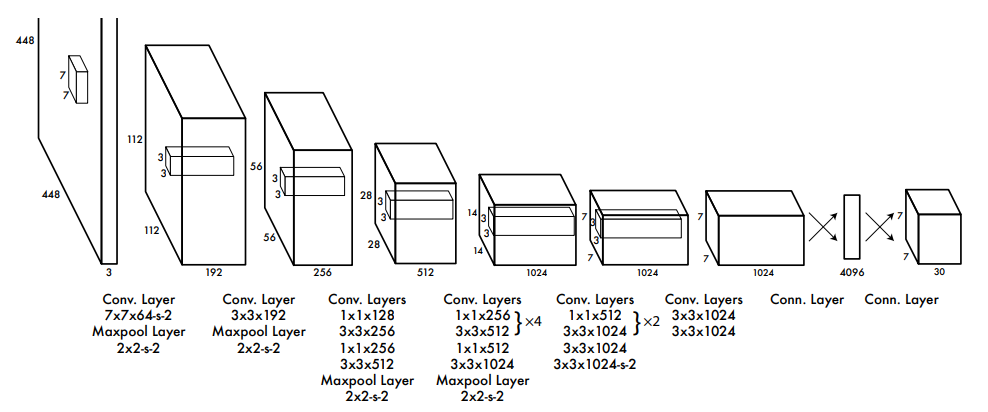
\includegraphics[width=0.4\textwidth]{figures/YOLOv1 Architecture.png}
    \caption{YOLOv1 Architecture}
    \label{fig:my_label}
\end{figure}


YOLOv1 architecture consists of 24 convolutional layers followed by two fully connected layers. In the paper, the authors took the first 20 convolutional layers from the backbone of the network and, with the addition of an average pooling layer and a single fully connected layer, where it was pre-trained and validated on the ImageNet 2012 dataset. During inference, the final four layers and 2 FC layers are added to the network; all initialized randomly.


\begin{figure}[h]
    \centering
    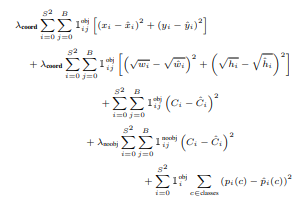
\includegraphics[width=0.4\textwidth]{figures/YOLO_Loss.png}
    \caption{YOLOv1 Loss function [reference to paper]}
    \label{fig:YOLO_Loss}
\end{figure}

YOLOv1 uses stochastic gradient descent as its optimizer; the Loss function is shown in Fig. 1. The Loss function comprises two parts, localization loss, and classification loss. The localization loss measures the error between the predicted bounding box coordinates and the ground-truth bounding box. The classification loss measures the error between the predicted class probabilities and the ground truth. The $\lambda_{coord}$ and $\lambda_{noobj}$ are regularization coefficients that regulate the magnitude of the different components, emphasizing object localization and deemphasizing grid cells without objects.  

\subsection{YOLOv5 Overview}

YOLOv5 is an object detection model that was first introduced in 2020 by Ultralytics, which builds on the success of previous YOLO models. YOLOv5 achieved SOTA performance on a variety of benchmark datasets while also being fast and efficient to train and deploy. YOLO made several architectural changes when YOLOv5 came around, most notably the standardized practice of structuring the model into three components, the backbone, the neck, and the head. 

\begin{figure}[h]
    \centering
    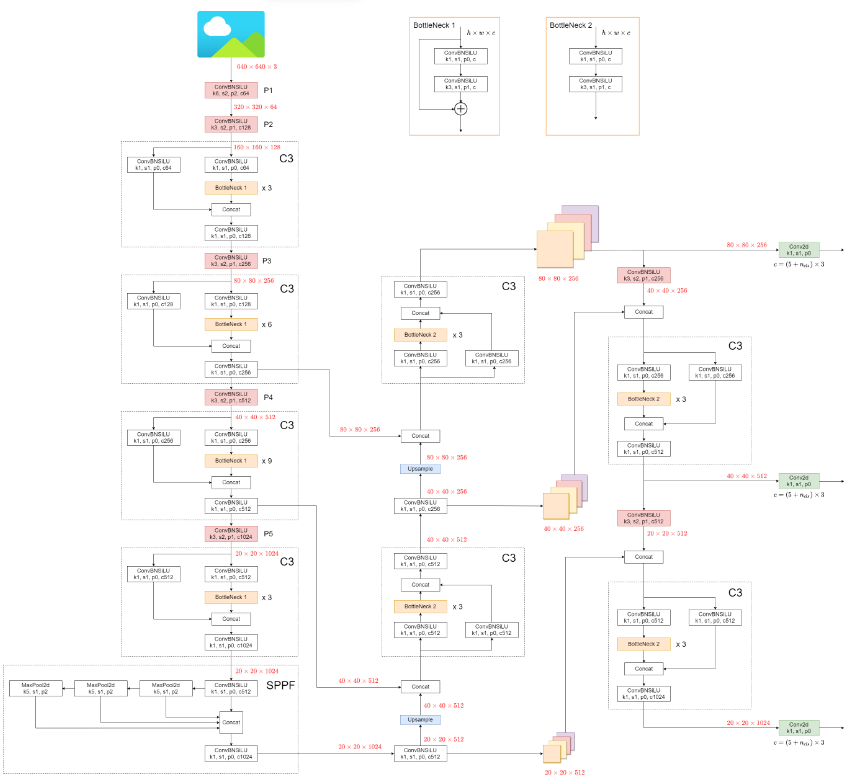
\includegraphics[width=0.4\textwidth]{figures/YOLOv5_arch.png}
    \caption{YOLOv5 Architecture}
    \label{fig:my_label}
\end{figure}

The backbone of YOLOv5 is a variant of Darknet53, a new network for performing feature extraction characterized by small filter windows and residual connections. YOLOv5 modifies Darknet 53 by introducing Cross Stage Partial (CSP) connections to the network. This enables the architecture to achieve a richer gradient combination while reducing the amount of computation. It involves dividing the backbone into two streams, one processing the image and another which processes a downsampled version of the input. They are later concatenated and passed to the next stage of the network. 

The neck of YOLOv5 is the Intermediate component that connects the backbone to the head. It aggregates and refines the features extracted by the backbone, often focusing on enhancing the spatial and semantic information across different scales. 

The first half of the neck is composed of a Spatial Pyramid Pooling (SPP) layer to remove the fixed-size constraint of the network, which is typically a requirement due to the final fully connected layers during the inference phase. This removes the need to warp, augment, or crop images, which generally change the aspect ratio and scale of the object in the image. 

The second half of the neck, the CSP-Path Aggregation Network (CSP-PAN), incorporates the features learned by the CSP blocks in the backbone and shortens the information path between lower layers and top features. PAN links the feature grid and all feature levels to make helpful information in each feature level propagate directly to subblocks. 

YOLOv5’s head consists of three branches, each predicting a different feature scale. In the original publication, the authors used different grid cell shapes for each level, especially grid cell sizes of 13 x 13, 26 x 26, and 52 x 52, with each grid cell predicting B = 3 bounding boxes. Each head produces bounding boxes, class probabilities, and confidence scores, with the output tensor being of shape S x S x (B x 5 + C), where 5 represents x, y, w, h, and the confidence score of the predicted class. Finally, the network uses Non-maximum Suppression (NMS) to filter out overlapping bounding boxes and only keep the most confident predictions.

YOLOv5 also incorporates anchor boxes, fixed-sized bounding boxes used to predict the location and size of objects within an image. Instead of predicting arbitrary bounding boxes for each object instance, the model predicts the coordinates of the anchor boxes with predefined aspect ratios and scales and adjusts them to fit the object instance.

\subsection{YOLOv8 Overview}
YOLOv8 is the latest version of the YOLO object detection model. This latest version has the same architecture as its predecessors \ref{fig:YOLOv8_arch} but it introduces numerous improvements compared to the earlier versions of YOLO such as a new neural network architecture that utilizes both Feature Pyramid Network (FPN) and Path Aggregation Network (PAN) and a new labeling tool that simplifies the annotation process. This labeling tool contains several useful features like auto labeling, labeling shortcuts, and customizable hotkeys. The combination of these features makes it easier to annotate images for training the model.
\begin{figure}[h]
    \centering
    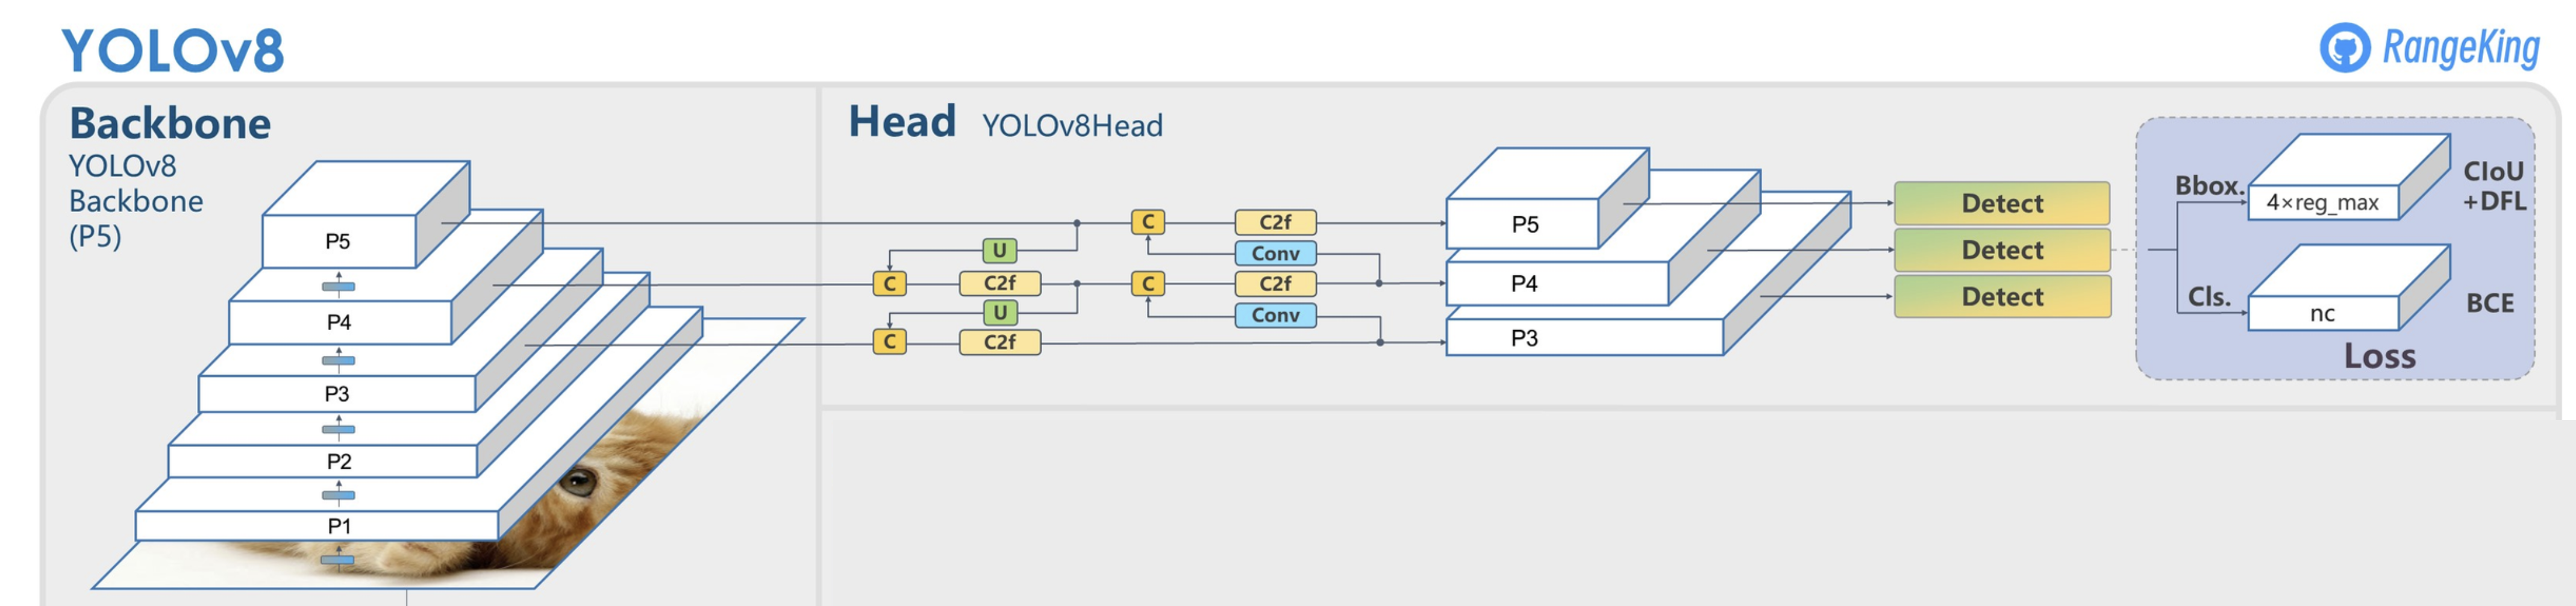
\includegraphics[width=0.4\textwidth]{figures/YOLOv8_arch.png}
    \caption{YOLOv8 Architecture [https://blog.roboflow.com/whats-new-in-yolov8/]}
    \label{fig:YOLOv8_arch}
\end{figure}
\\
The FPN works by gradually reducing the spatial resolution of the input image while increasing the number of feature channels. This results in the creation of feature maps that are capable of detecting objects at different scales and resolutions. The PAN architecture, on the other hand, aggregates features from different levels of the network through skip connections. By doing so, the network can better capture features at multiple scales and resolutions, which is crucial for accurately detecting objects of different sizes and shapes.[https://arxiv.org/pdf/2304.00501.pdf]\\

\subsection{YOLOv8 vs YOLOv5}
Both YOLOv5 and YOLOv8 use mosaic augmentation on the training set. Mosaic augmentation is a data augmentation technique that takes four random images from the training set and combines them into a single mosaic image. This image, where each quadrant contains a random crop from one of the four input images, is then inputted into the model [https://blog.roboflow.com/advanced-augmentations/]\\
One of the key differences between YOLOv8 and YOLOv5 is their neural network architectures. YOLOv8 uses a new architecture that combines both Feature Pyramid Network (FPN) and Path Aggregation Network (PAN) modules, while YOLOv5 uses a modified version of the CSPDarknet architecture. FPN is used to generate feature maps at multiple scales and resolutions, while PAN is used to aggregate features from different levels of the network to improve accuracy.\\
Performance: YOLOv8 is generally considered to be more accurate than YOLOv5. In benchmark tests, YOLOv8 has achieved higher mean Average Precision (mAP) scores than YOLOv5 on several datasets, particularly for small objects and objects with complex shapes.\\
Training data: YOLOv8 was trained on a larger and more diverse dataset than YOLOv5, which can lead to better performance on a wider range of images. YOLOv8 was trained on a combination of the COCO dataset and several other datasets, while YOLOv5 was trained primarily on the COCO dataset.\\
Labeling tool: YOLOv8 includes a new labeling tool called RoboFlow Annotate that makes it easier to annotate images for training the model. The tool includes several features such as auto labeling, labeling shortcuts, and customizable hotkeys. In contrast, YOLOv5 uses a different labeling tool.\\
Post-processing: YOLOv8 includes more advanced post-processing techniques than YOLOv5, which can help to filter out false positives and improve the accuracy of the final detections. For example, YOLOv8 uses a technique called Soft-NMS to filter out redundant bounding boxes, while YOLOv5 uses a simpler NMS algorithm.\\
Object detection speed: YOLOv8 is slightly slower than YOLOv5 in terms of object detection speed. However, YOLOv8 is still able to process images in real-time on modern GPUs.\\
Outpt heads: YOLOv5 has 3 output heads while YOLOv8 has 1 output head. YOLOv8 Does not have small, medium, and large anchor boxes rather it uses an anchor free detection mechanism that predicts directly the center of an object instead of the offset from a known anchor box which reduces the number of box predictions, and that speeds up Non-Maximum Suppression (NMS), which is a complicated post processing step that sifts through candidate detections after inference.\\
Overall, YOLOv8 introduces several improvements over YOLOv5, particularly in terms of neural network architecture, performance, and post-processing techniques. These improvements have resulted in significantly higher accuracy and better performance for object detection, making YOLOv8 a popular choice for a wide range of computer vision applications.\\

%---------------------------------------------------------------------
\section{Model Evaluation}

\begin{figure}[h]
    \centering
    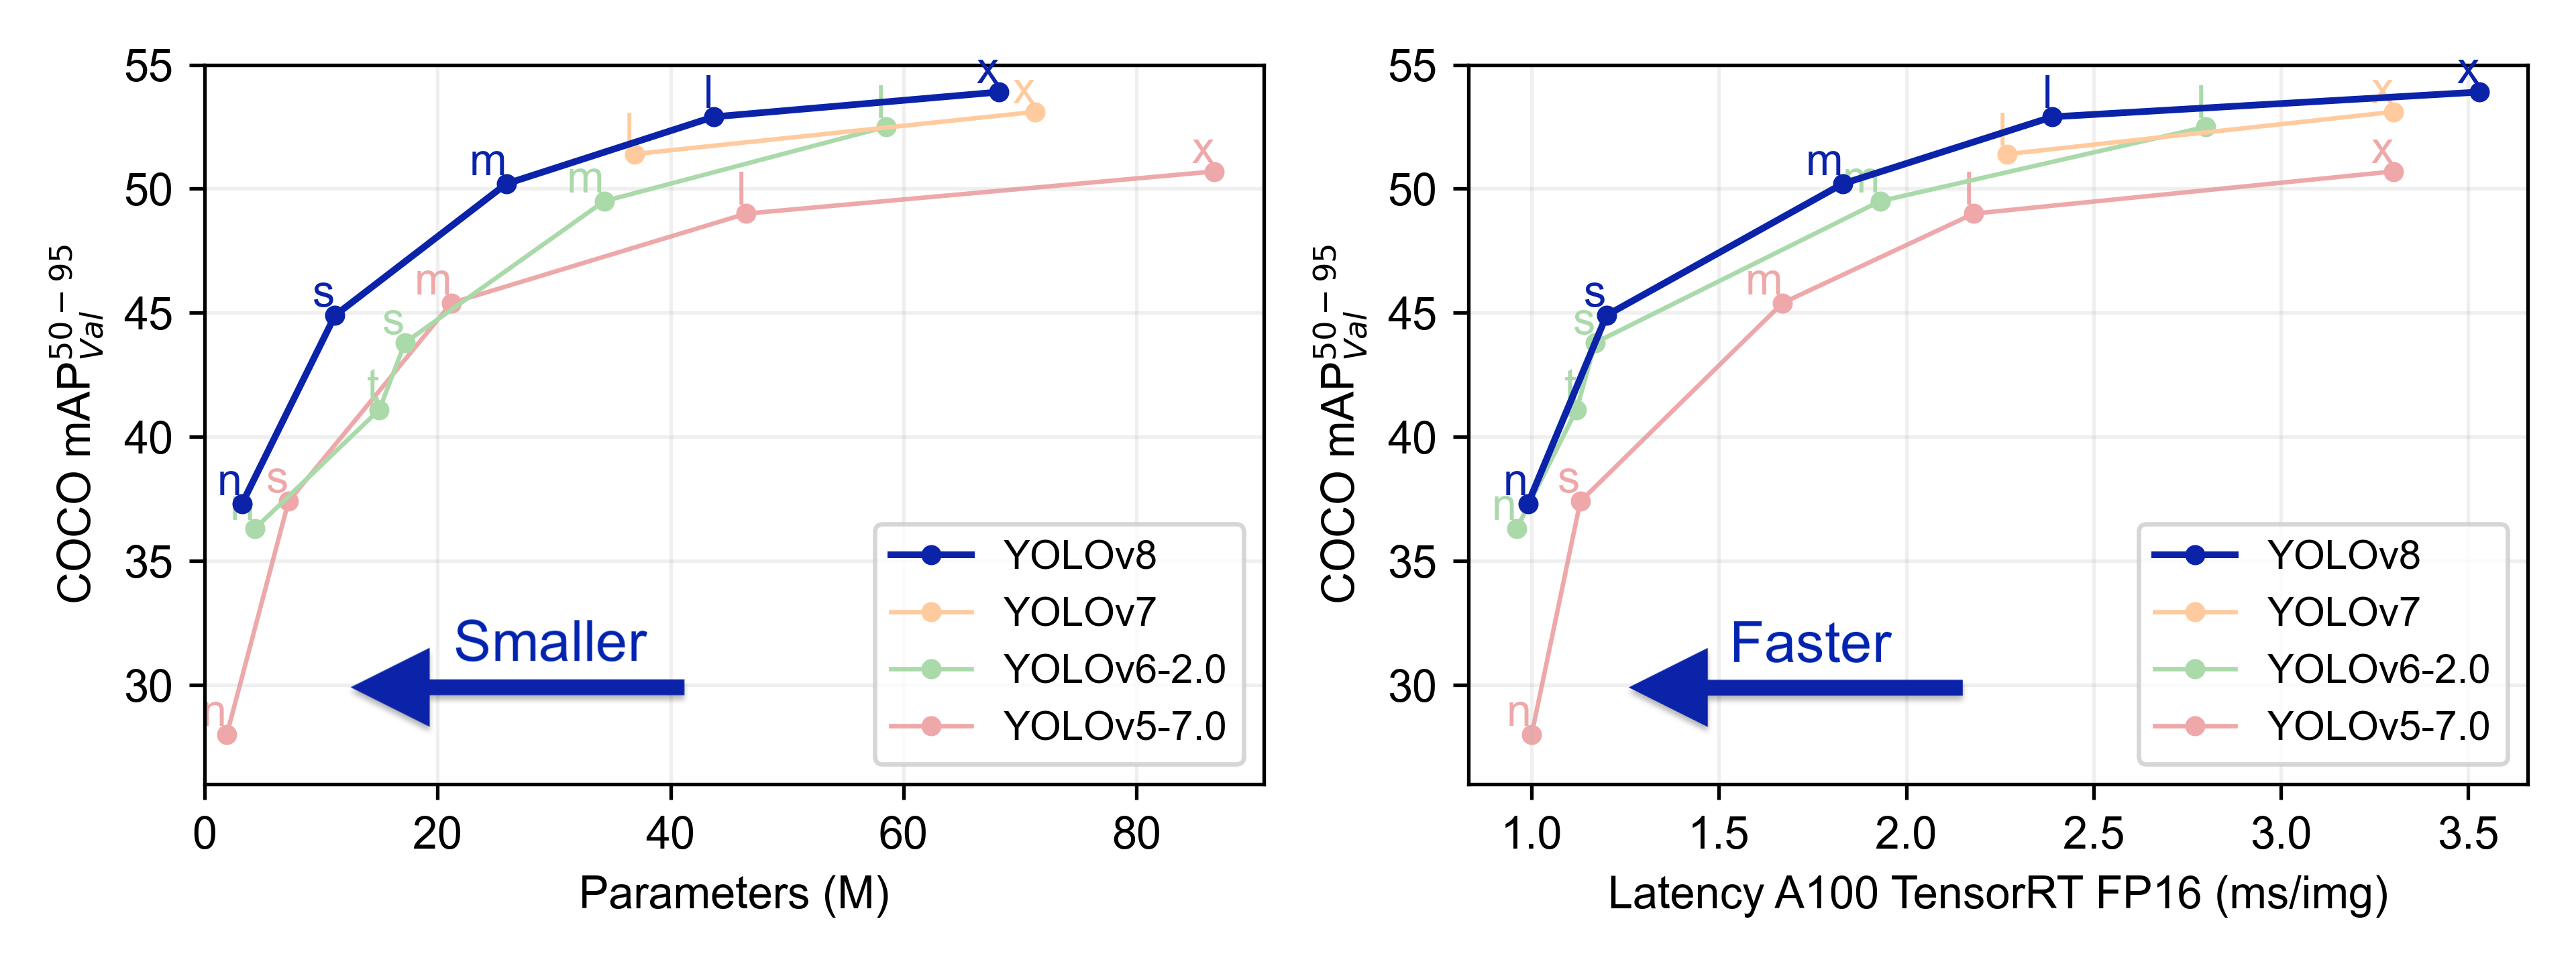
\includegraphics[width=0.45\textwidth]{figures/yolo-comparison-plots.png}
    \caption{Shows the performance of each YOLO model and it's respective versions for mAP50 against number of parameters and inference speed}
    \label{fig:my_label}
\end{figure}

Mean Average Precision (mAP) is a commonly used evaluation metric for object detection that combines Precision, recall, IOU, and AP. Precision is the ratio of true positives to the total number of detections. At the same time, recall is the ratio of true positives to the total number of ground truth objects in an image. Recall values range from 0.0 to 1.0 with a stepsize of 0.1. In contrast, the interpolated precision value is defined as the maximum Precision corresponding to the recall value more significant than the current recall value. The curve we obtain is commonly called the precision-recall curve. Average Precision is therefore defined as the area underneath this curve. A higher AP score indicates better performance since it means the model is accurately detecting more objects in an image while minimizing false positives. 

It is essential to define what we consider a valid detection by our model. mAP50 uses IoU as its threshold parameter, defined as an area of overlap over an area of union between the predicted bounding box and ground truth, set at an IoU = 50\% or greater. Finally, we average the result APs over all the category classes to obtain mAP50. mAP50:95 corresponds to the average mAP across all categories for different IoU thresholds, starting from 50% to 95%, with a step size of 5\%. This provides a more comprehensive evaluation of the model’s performance across various confidence levels.

% \par
% \begin{table}[h]
% \begin{center}
% \scalebox{0.9}{
% \begin{tabular}{|l|c|c|c|}
% \hline
% Model   & \multicolumn{1}{l|}{Parameters (M)} & \multicolumn{1}{l|}{Inference (ms)} & \multicolumn{1}{l|}{mAP50:95} \\ \hline
% YOLOv8n & \cellcolor[HTML]{FFFFFF}3.2         & \cellcolor[HTML]{FFFFFF}0.99        & \cellcolor[HTML]{FFFFFF}37.3  \\ \hline
% YOLOv8s & \cellcolor[HTML]{FFFFFF}11.2        & \cellcolor[HTML]{FFFFFF}1.20        & \cellcolor[HTML]{FFFFFF}44.9  \\ \hline
% YOLOv8m & \cellcolor[HTML]{FFFFFF}25.9        & \cellcolor[HTML]{FFFFFF}1.83        & \cellcolor[HTML]{FFFFFF}50.2  \\ \hline
% YOLOv8l & \cellcolor[HTML]{FFFFFF}43.7        & \cellcolor[HTML]{FFFFFF}2.39        & \cellcolor[HTML]{FFFFFF}52.9  \\ \hline
% YOLOv8x & \cellcolor[HTML]{FFFFFF}68.2        & \cellcolor[HTML]{FFFFFF}3.53        & \cellcolor[HTML]{FFFFFF}53.9  \\ \hline
% \end{tabular}
% }
% \end{center}
% \caption{YOLOv8 models pre-trained on the COCO val2017 dataset. Inference speed is averaged over COCO class images using an Amazon EC2 P4d instance}
% \end{table}

\begin{figure}[h]
    \centering
    \subfloat[\centering Confusion matrix for the different classes]{{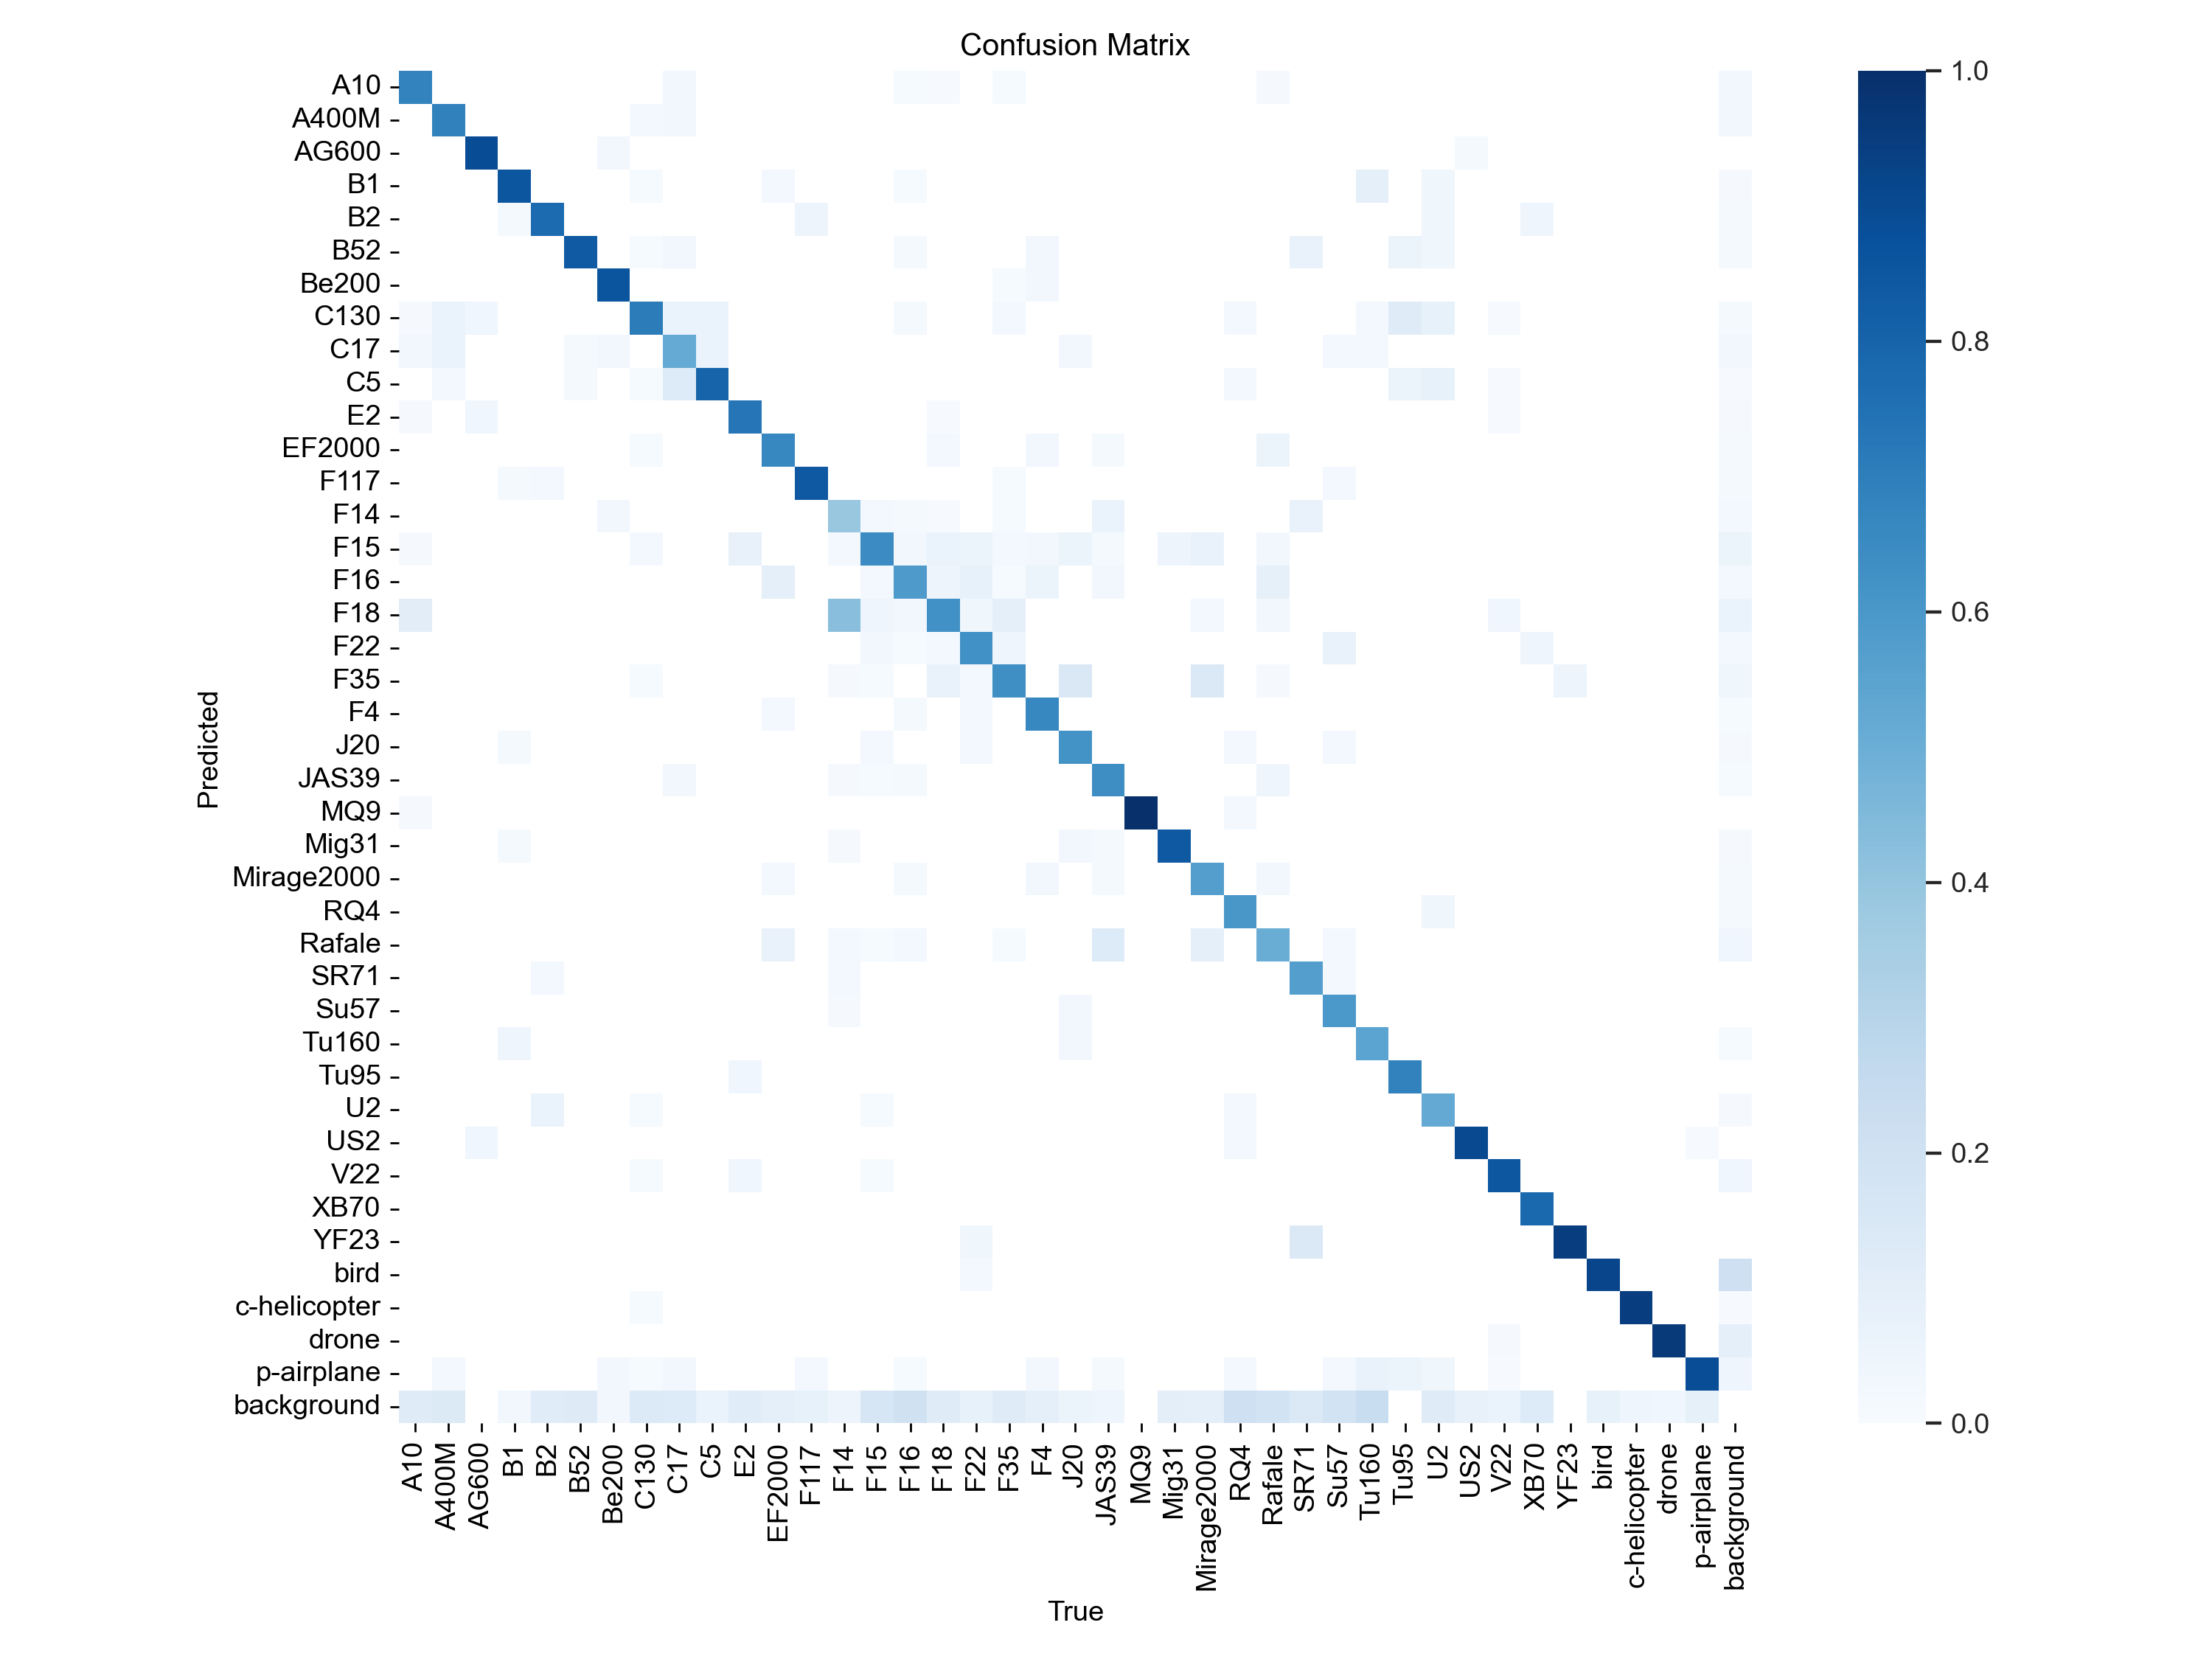
\includegraphics[width=3.2cm]{figures/confusion_matrix.png}}}
    \qquad
    \subfloat[\centering PR curve showing for each individual class and overall]{{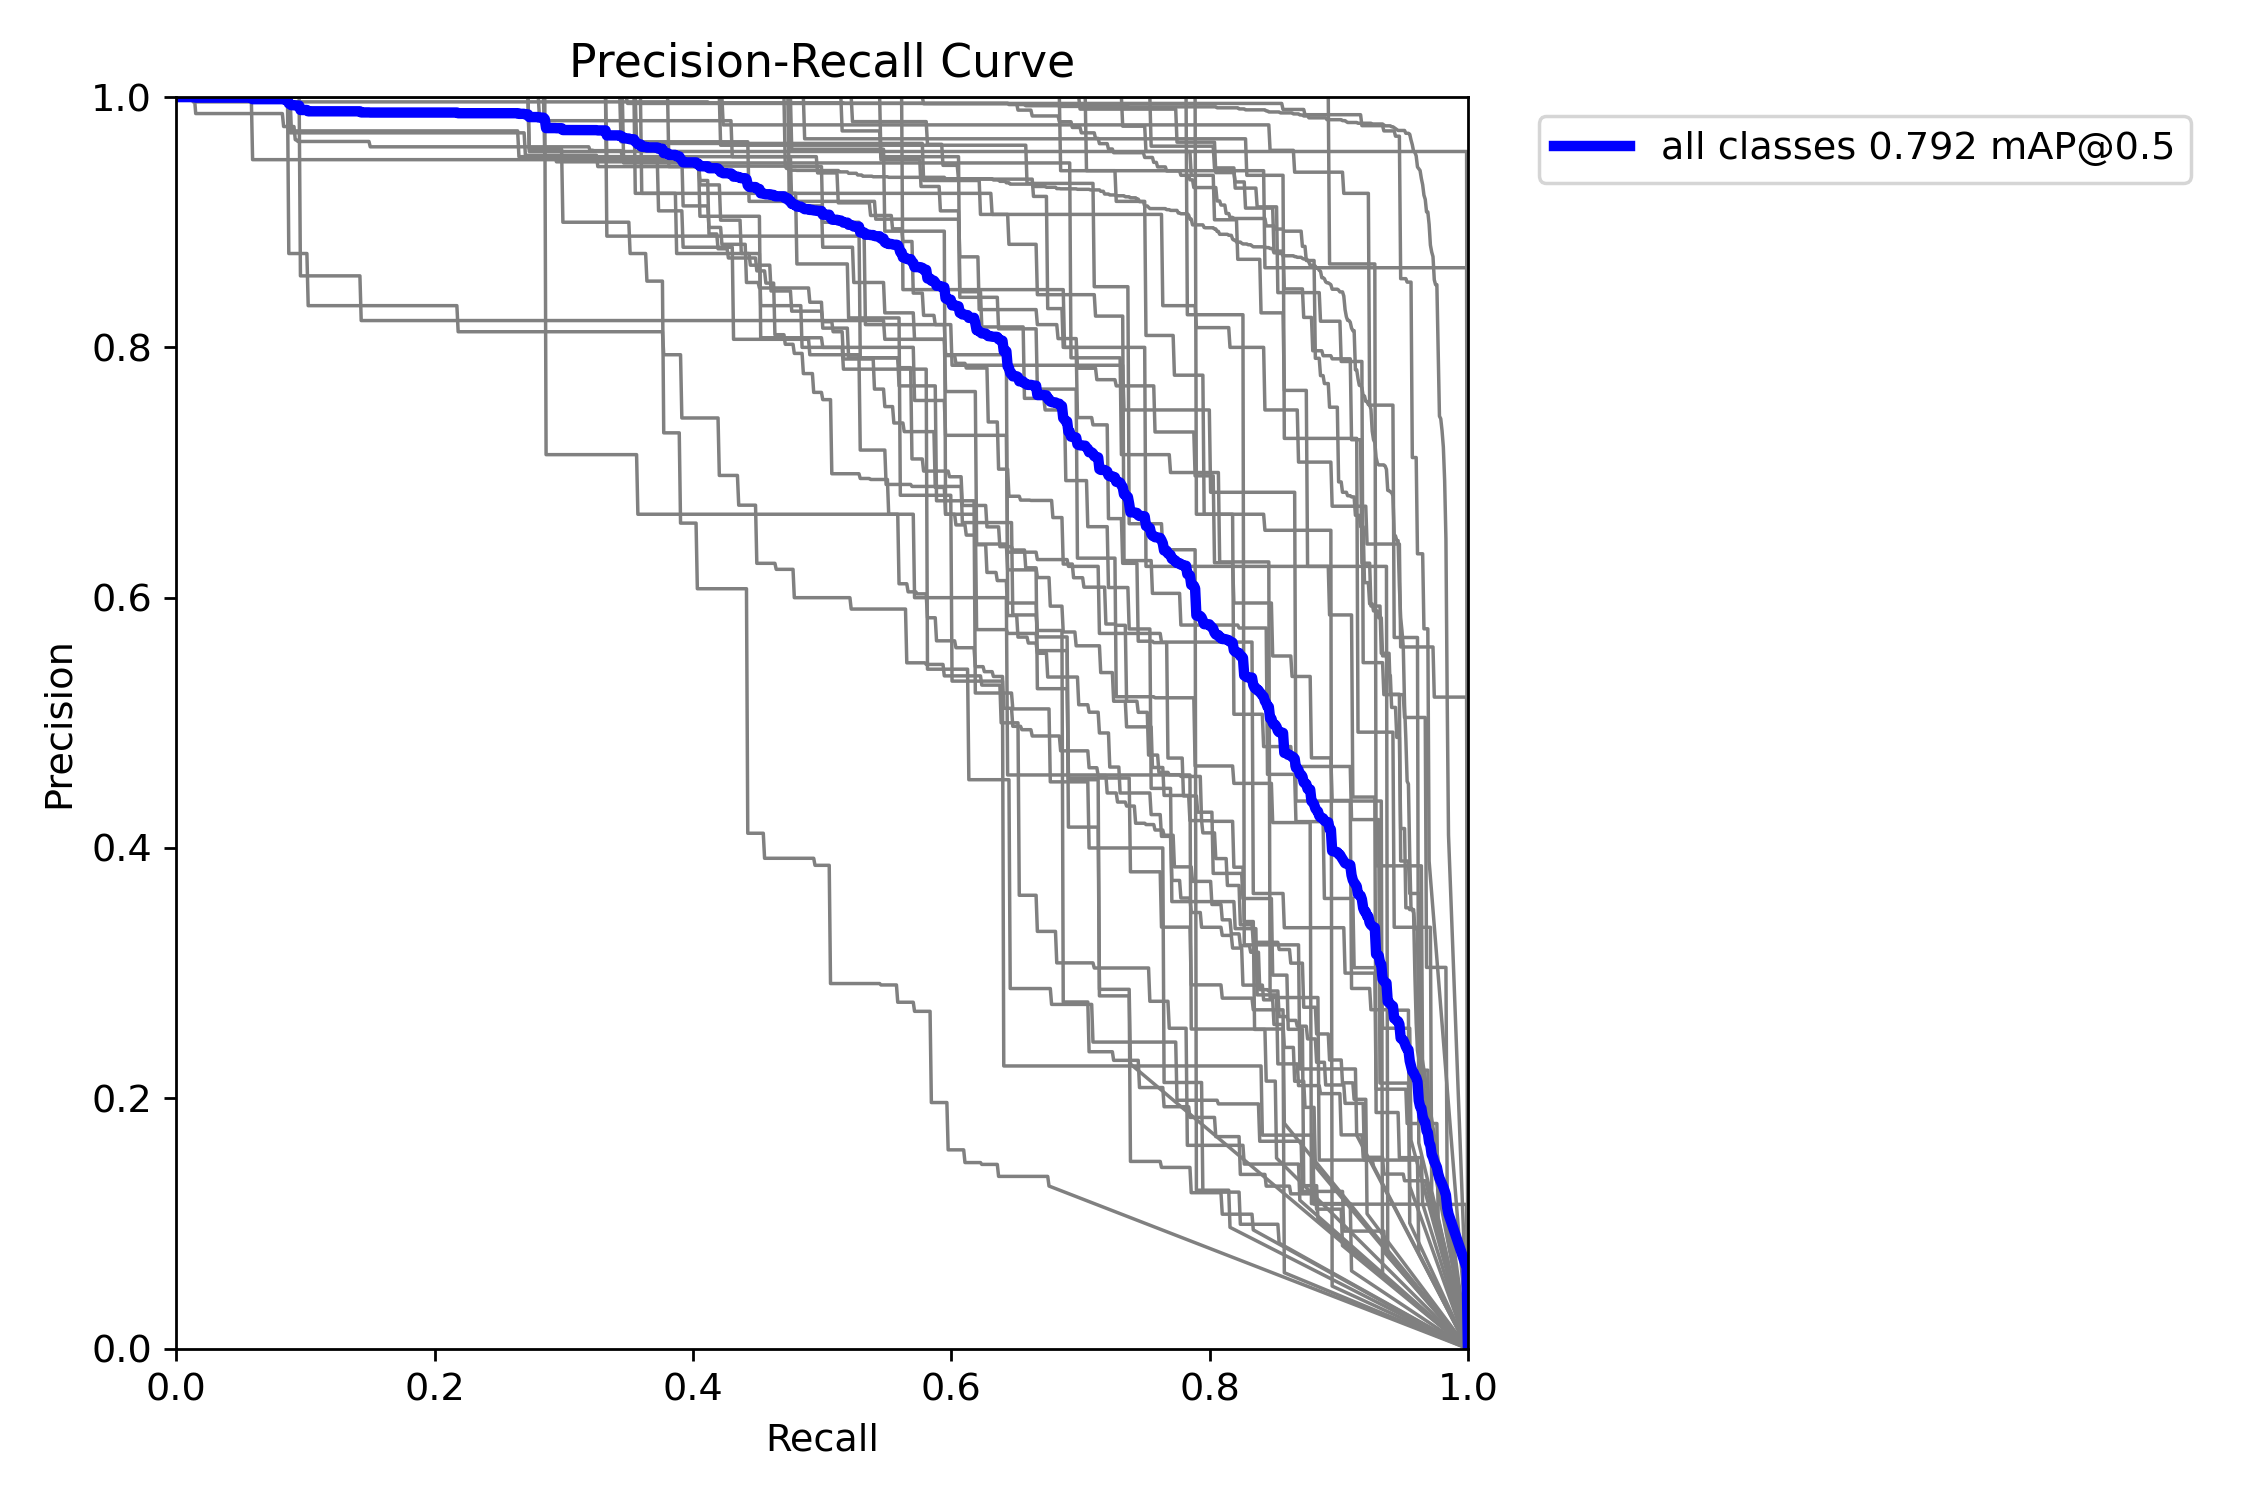
\includegraphics[width=3.5cm]{PR_curve.png} }}%
    \caption{TBA}%
    \label{fig:example}
\end{figure}

The model we performed our evaluation on was the YOLOv8m model, which was trained on the flying object detection dataset, saw a mAP@50 = 79.2\% and mAP@50:95 = 68.5\%. Performance was relatively stable across most classes according to the confusion matrix in Fig. 5. 

\subsection{Low Intraclass Variance Discussion}

Classes that are similar to each other in an object detection algorithm can pose a challenge for the model as it may struggle to distinguish between the two classes. For example, if the dataset we use contains many different families of planes which the model may have difficulty distinguishing between them. This problem is often called class confusion and can typically effect models object detection models.

To combat this problem, one approach is to view a confusion matrix, which visualizes the number of predicted classes versus the ground truth label. Looking at our confusion matrix in Fig. 5, the model does surprisingly well for low intraclass variance categories, such as the "fighter" family. 

We attempt to take the most visually striking


\section{Miscellaneous Information}

The rest of the information in this format template has been adapted from CVPR 2020 and provides guidelines on the lower-level specifications regarding the paper's format.

\subsection{Language}

All manuscripts must be in English.


\subsection{Paper length}
Papers, excluding the references section,
must be no longer than six pages in length. The references section
will not be included in the page count, and there is no limit on the
length of the references section. For example, a paper of six pages
with two pages of references would have a total length of 8 pages.

%-------------------------------------------------------------------------
\subsection{The ruler}
The \LaTeX\ style defines a printed ruler which should be present in the
version submitted for review.  The ruler is provided in order that
reviewers may comment on particular lines in the paper without
circumlocution.  If you are preparing a document using a non-\LaTeX\
document preparation system, please arrange for an equivalent ruler to
appear on the final output pages.  The presence or absence of the ruler
should not change the appearance of any other content on the page.  The
camera ready copy should not contain a ruler. (\LaTeX\ users may uncomment
the \verb'\cvprfinalcopy' command in the document preamble.)  Reviewers:
note that the ruler measurements do not align well with lines in the paper
--- this turns out to be very difficult to do well when the paper contains
many figures and equations, and, when done, looks ugly.  Just use fractional
references (e.g.\ this line is $095.5$), although in most cases one would
expect that the approximate location will be adequate.

\subsection{Mathematics}

Please number all of your sections and displayed equations.  It is
important for readers to be able to refer to any particular equation.  Just
because you didn't refer to it in the text doesn't mean some future reader
might not need to refer to it.  It is cumbersome to have to use
circumlocutions like ``the equation second from the top of page 3 column
1''.  (Note that the ruler will not be present in the final copy, so is not
an alternative to equation numbers).  All authors will benefit from reading
Mermin's description of how to write mathematics:
\url{http://www.pamitc.org/documents/mermin.pdf}.

Finally, you may feel you need to tell the reader that more details can be
found elsewhere, and refer them to a technical report.  For conference
submissions, the paper must stand on its own, and not {\em require} the
reviewer to go to a techreport for further details.  Thus, you may say in
the body of the paper ``further details may be found
in~\cite{Authors14b}''.  Then submit the techreport as additional material.
Again, you may not assume the reviewers will read this material.

Sometimes your paper is about a problem which you tested using a tool which
is widely known to be restricted to a single institution.  For example,
let's say it's 1969, you have solved a key problem on the Apollo lander,
and you believe that the CVPR70 audience would like to hear about your
solution.  The work is a development of your celebrated 1968 paper entitled
``Zero-g frobnication: How being the only people in the world with access to
the Apollo lander source code makes us a wow at parties'', by Zeus \etal.

You can handle this paper like any other.  Don't write ``We show how to
improve our previous work [Anonymous, 1968].  This time we tested the
algorithm on a lunar lander [name of lander removed for blind review]''.
That would be silly, and would immediately identify the authors. Instead
write the following:
\begin{quotation}
\noindent
   We describe a system for zero-g frobnication.  This
   system is new because it handles the following cases:
   A, B.  Previous systems [Zeus et al. 1968] didn't
   handle case B properly.  Ours handles it by including
   a foo term in the bar integral.

   ...

   The proposed system was integrated with the Apollo
   lunar lander, and went all the way to the moon, don't
   you know.  It displayed the following behaviours
   which show how well we solved cases A and B: ...
\end{quotation}
As you can see, the above text follows standard scientific convention,
reads better than the first version, and does not explicitly name you as
the authors.  A reviewer might think it likely that the new paper was
written by Zeus \etal, but cannot make any decision based on that guess.
He or she would have to be sure that no other authors could have been
contracted to solve problem B.
\medskip

\noindent
FAQ\medskip\\
{\bf Q:} Are acknowledgements OK?\\
{\bf A:} No.  Leave them for the final copy.\medskip\\
{\bf Q:} How do I cite my results reported in open challenges?
{\bf A:} To conform with the double blind review policy, you can report results of other challenge participants together with your results in your paper. For your results, however, you should not identify yourself and should not mention your participation in the challenge. Instead present your results referring to the method proposed in your paper and draw conclusions based on the experimental comparison to other results.\medskip\\

\begin{figure}[t]
\begin{center}
\fbox{\rule{0pt}{2in} \rule{0.9\linewidth}{0pt}}
   %\includegraphics[width=0.8\linewidth]{egfigure.eps}
\end{center}
   \caption{Example of caption.  It is set in Roman so that mathematics
   (always set in Roman: $B \sin A = A \sin B$) may be included without an
   ugly clash.}
\label{fig:long}
\label{fig:onecol}
\end{figure}

\subsection{Miscellaneous}

\noindent
Compare the following:\\
\begin{tabular}{ll}
 \verb'$conf_a$' &  $conf_a$ \\
 \verb'$\mathit{conf}_a$' & $\mathit{conf}_a$
\end{tabular}\\
See The \TeX book, p165.

The space after \eg, meaning ``for example'', should not be a
sentence-ending space. So \eg is correct, {\em e.g.} is not.  The provided
\verb'\eg' macro takes care of this.

When citing a multi-author paper, you may save space by using ``et alia'',
shortened to ``\etal'' (not ``{\em et.\ al.}'' as ``{\em et}'' is a complete word.)
However, use it only when there are three or more authors.  Thus, the
following is correct: ``
   Frobnication has been trendy lately.
   It was introduced by Alpher~\cite{Alpher02}, and subsequently developed by
   Alpher and Fotheringham-Smythe~\cite{Alpher03}, and Alpher \etal~\cite{Alpher04}.''

This is incorrect: ``... subsequently developed by Alpher \etal~\cite{Alpher03} ...''
because reference~\cite{Alpher03} has just two authors.  If you use the
\verb'\etal' macro provided, then you need not worry about double periods
when used at the end of a sentence as in Alpher \etal.

For this citation style, keep multiple citations in numerical (not
chronological) order, so prefer \cite{Alpher03,Alpher02,Authors14} to
\cite{Alpher02,Alpher03,Authors14}.


\begin{figure*}
\begin{center}
\fbox{\rule{0pt}{2in} \rule{.9\linewidth}{0pt}}
\end{center}
   \caption{Example of a short caption, which should be centered.}
\label{fig:short}
\end{figure*}

%------------------------------------------------------------------------
\subsection{Formatting your paper}

All text must be in a two-column format. The total allowable width of the
text area is $6\frac78$ inches (17.5 cm) wide by $8\frac78$ inches (22.54
cm) high. Columns are to be $3\frac14$ inches (8.25 cm) wide, with a
$\frac{5}{16}$ inch (0.8 cm) space between them. The main title (on the
first page) should begin 1.0 inch (2.54 cm) from the top edge of the
page. The second and following pages should begin 1.0 inch (2.54 cm) from
the top edge. On all pages, the bottom margin should be 1-1/8 inches (2.86
cm) from the bottom edge of the page for $8.5 \times 11$-inch paper; for A4
paper, approximately 1-5/8 inches (4.13 cm) from the bottom edge of the
page.

%-------------------------------------------------------------------------
\subsection{Margins and page numbering}

All printed material, including text, illustrations, and charts, must be kept
within a print area 6-7/8 inches (17.5 cm) wide by 8-7/8 inches (22.54 cm)
high.



%-------------------------------------------------------------------------
\subsection{Type-style and fonts}

Wherever Times is specified, Times Roman may also be used. If neither is
available on your word processor, please use the font closest in
appearance to Times to which you have access.

MAIN TITLE. Center the title 1-3/8 inches (3.49 cm) from the top edge of
the first page. The title should be in Times 14-point, boldface type.
Capitalize the first letter of nouns, pronouns, verbs, adjectives, and
adverbs; do not capitalize articles, coordinate conjunctions, or
prepositions (unless the title begins with such a word). Leave two blank
lines after the title.

AUTHOR NAME(s) and AFFILIATION(s) are to be centered beneath the title
and printed in Times 12-point, non-boldface type. This information is to
be followed by two blank lines.

The ABSTRACT and MAIN TEXT are to be in a two-column format.

MAIN TEXT. Type main text in 10-point Times, single-spaced. Do NOT use
double-spacing. All paragraphs should be indented 1 pica (approx. 1/6
inch or 0.422 cm). Make sure your text is fully justified---that is,
flush left and flush right. Please do not place any additional blank
lines between paragraphs.

Figure and table captions should be 9-point Roman type as in
Figures~\ref{fig:onecol} and~\ref{fig:short}.  Short captions should be centred.

\noindent Callouts should be 9-point Helvetica, non-boldface type.
Initially capitalize only the first word of section titles and first-,
second-, and third-order headings.

FIRST-ORDER HEADINGS. (For example, {\large \bf 1. Introduction})
should be Times 12-point boldface, initially capitalized, flush left,
with one blank line before, and one blank line after.

SECOND-ORDER HEADINGS. (For example, { \bf 1.1. Database elements})
should be Times 11-point boldface, initially capitalized, flush left,
with one blank line before, and one after. If you require a third-order
heading (we discourage it), use 10-point Times, boldface, initially
capitalized, flush left, preceded by one blank line, followed by a period
and your text on the same line.

%-------------------------------------------------------------------------
\subsection{Footnotes}

Please use footnotes\footnote {This is what a footnote looks like.  It
often distracts the reader from the main flow of the argument.} sparingly.
Indeed, try to avoid footnotes altogether and include necessary peripheral
observations in
the text (within parentheses, if you prefer, as in this sentence).  If you
wish to use a footnote, place it at the bottom of the column on the page on
which it is referenced. Use Times 8-point type, single-spaced.


%-------------------------------------------------------------------------
\subsection{References}

List and number all bibliographical references in 9-point Times,
single-spaced, at the end of your paper. When referenced in the text,
enclose the citation number in square brackets, for
example~\cite{Authors14}.  Where appropriate, include the name(s) of
editors of referenced books.

\begin{table}
\begin{center}
\begin{tabular}{|l|c|}
\hline
Method & Frobnability \\
\hline\hline
Theirs & Frumpy \\
Yours & Frobbly \\
Ours & Makes one's heart Frob\\
\hline
\end{tabular}
\end{center}
\caption{Results.   Ours is better.}
\end{table}

%-------------------------------------------------------------------------
\subsection{Illustrations, graphs, and photographs}

All graphics should be centered.  Please ensure that any point you wish to
make is resolvable in a printed copy of the paper.  Resize fonts in figures
to match the font in the body text, and choose line widths which render
effectively in print.  Many readers (and reviewers), even of an electronic
copy, will choose to print your paper in order to read it.  You cannot
insist that they do otherwise, and therefore must not assume that they can
zoom in to see tiny details on a graphic.

When placing figures in \LaTeX, it's almost always best to use
\verb+\includegraphics+, and to specify the  figure width as a multiple of
the line width as in the example below
{\small\begin{verbatim}
   \usepackage[dvips]{graphicx} ...
   \includegraphics[width=0.8\linewidth]
                   {myfile.eps}
\end{verbatim}
}


%-------------------------------------------------------------------------
\subsection{Color}

Please refer to the author guidelines on the CVPR 2020 web page for a discussion
of the use of color in your document.

%------------------------------------------------------------------------

%-------------------------------------------------------------------------


{\small
\bibliographystyle{ieee_fullname}
\bibliography{egbib}
}
% \begin{figure}[]
%   \centering
%   \begin{subfigure}[b]{0.45\linewidth}
%     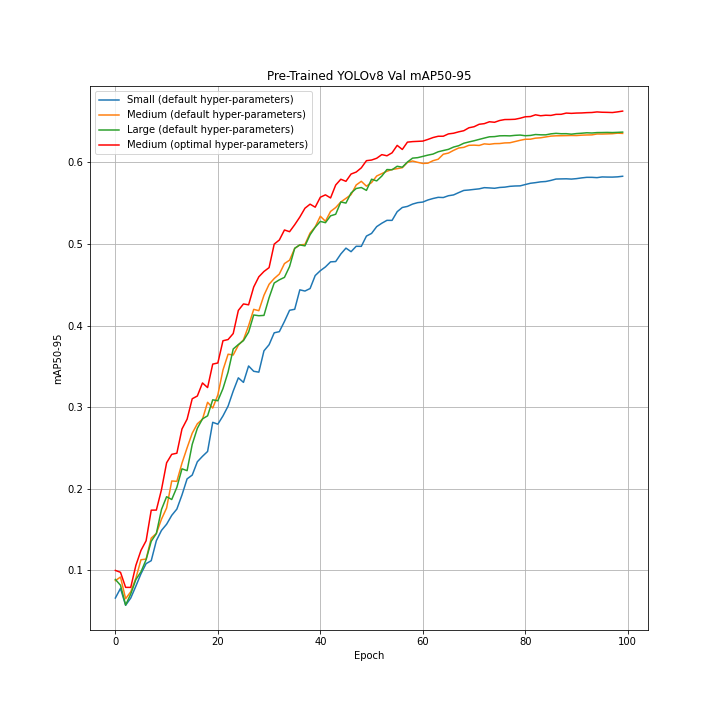
\includegraphics[width=\linewidth]{figures/Pre-Trained YOLOv8 Val mAP50-95.png}
%     \caption{Pre-Trained YOLOv8 Val mAP50-95}
%     \label{fig:YOLOv8_mAP50-95_val}
%   \end{subfigure}
%   \hspace{0.07\linewidth}
%   \begin{subfigure}[b]{0.45\linewidth}
%     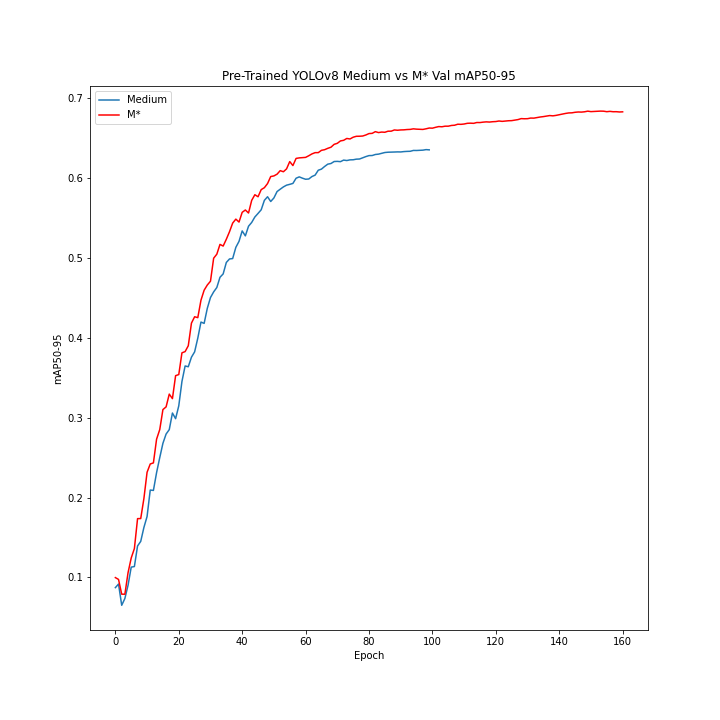
\includegraphics[width=\linewidth]{figures/Pre-Trained YOLOv8 Medium vs Mstar Val mAP50-95.png}
%     \caption{Pre-Trained YOLOv8 Medium vs M* Val mAP50-95}
%     \label{fig:M_mAP50-95_val}
%   \end{subfigure}
%   \caption{Two plots side by side}
%   \label{fig:plots}
% \end{figure}

% \begin{table}[]
%     \centering
%     \begin{tabular}{|c|ccc|}
%         \hline
%          & train/box\textunderscore loss & train/cls\textunderscore loss & train/dfl\textunderscore loss \\
%          \hline
%         b16\textunderscore sgd\textunderscore cls1\textunderscore box5.5\textunderscore dfl2.5 & 0.79816 & 2.4675 & 1.9951 \\
%         b16\textunderscore sgd\textunderscore cls1.5\textunderscore box5.5\textunderscore dfl3 & 0.8061 & 3.6908 & 2.413 \\
%         b16\textunderscore sgd\textunderscore cls1\textunderscore box5.5\textunderscore dfl2 & 0.8026 & 2.4756 & 1.6047 \\
%         b16\textunderscore sgd\textunderscore cls1\textunderscore box6.5\textunderscore dfl2.5 & 0.94334 & 2.4827 & 1.992 \\
%         b16\textunderscore sgd\textunderscore cls1\textunderscore box6.5\textunderscore dfl2 & 0.94538 & 2.499 & 1.6052 \\
%         b16\textunderscore sgd\textunderscore cls1 & 1.0946 & 2.4923 & 1.2087 \\
%         b16\textunderscore sgd\textunderscore cls0.75 & 1.0883 & 1.8881 & 1.2036 \\
%         b16\textunderscore sgd\textunderscore cls1.5 & 1.1032 & 3.694 & 1.2088 \\
%         b16\textunderscore sgd\textunderscore cls1.5\textunderscore box5.5\textunderscore dfl2.5 & 1.1032 & 3.694 & 1.2088 \\
%         b16\textunderscore sgd\textunderscore cls0.5 & 1.0917 & 1.3071 & 1.2086 \\
%         b8\textunderscore sgd\textunderscore cls0.75 & 1.102 & 1.9914 & 1.2253 \\
%         b8\textunderscore sgd\textunderscore cls0.5 & 1.1044 & 1.3781 & 1.2273 \\
%         b16\textunderscore adam\textunderscore cls0.75 & 1.3592 & 3.2311 & 1.4455 \\
%         b16\textunderscore adam\textunderscore cls0.5 & 1.3595 & 2.2394 & 1.4554 \\
%         b16\textunderscore RMSProp\textunderscore cls0.5 & 2.0057 & 3.2682 & 1.9874 \\
%         b16\textunderscore RMSProp\textunderscore cls0.75 & 1.9559 & 4.6764 & 1.8572 \\
%         \hline
%     \end{tabular}
%     \caption{Hyperparameter tuning training loss}
%     \label{tab:Hyper_param_tune_1_1}
% \end{table}
% \begin{table}[]
%     \centering
%     \begin{tabular}{|c|ccc|}
%         \hline
%          & val/box\textunderscore loss & val/cls\textunderscore loss & val/dfl\textunderscore loss \\
%          \hline
%         b16\textunderscore sgd\textunderscore cls1\textunderscore box5.5\textunderscore dfl2.5 & 0.81255 & 2.0867 & 1.9262  \\
%         b16\textunderscore sgd\textunderscore cls1.5\textunderscore box5.5\textunderscore dfl3 & 0.83359 & 3.183 & 2.3506 \\
%         b16\textunderscore sgd\textunderscore cls1\textunderscore box5.5\textunderscore dfl2 & 0.82317 & 2.1138	1.5581 \\
%         b16\textunderscore sgd\textunderscore cls1\textunderscore box6.5\textunderscore dfl2.5 & 0.97155 & 2.1407 & 1.9295 \\
%         b16\textunderscore sgd\textunderscore cls1\textunderscore box6.5\textunderscore dfl2 & 0.97468 & 2.1111	1.5615 \\
%         b16\textunderscore sgd\textunderscore cls1 & 1.1371	2.1358 & 1.1697 \\
%         b16\textunderscore sgd\textunderscore cls0.75 & 1.1176 & 1.6147 & 1.1677 \\
%         b16\textunderscore sgd\textunderscore cls1.5 & 1.1484 & 3.313 & 1.1862 \\
%         b16\textunderscore sgd\textunderscore cls1.5\textunderscore box5.5\textunderscore dfl2.5 & 1.1484	3.313 & 1.1862 \\
%         b16\textunderscore sgd\textunderscore cls0.5 & 1.1133 & 1.1086 & 1.1689 \\
%         b8\textunderscore sgd\textunderscore cls0.75 & 1.1138 & 1.6773 & 1.1819 \\
%         b8\textunderscore sgd\textunderscore cls0.5 & 1.1075 & 1.1308	1.1784 \\
%         b16\textunderscore adam\textunderscore cls0.75 & 1.3698	2.7459 & 1.4342 \\
%         b16\textunderscore adam\textunderscore cls0.5 & 1.3736 & 1.8825 & 1.4454 \\
%         b16\textunderscore RMSProp\textunderscore cls0.5 & 4.0705 & 6.3487 & 3.5195 \\
%         b16\textunderscore RMSProp\textunderscore cls0.75 & 4.0336 & 29.961 & 3.7351 \\
%         \hline
%     \end{tabular}
%     \caption{Hyperparameter tuning validation loss}
%     \label{tab:Hyper_param_tune_1_2}
% \end{table}
% -------------------------------------------------------------------------------
\section {Annoying plots}

\begin{table*}
\begin{center}
    \begin{tabular}{|l|cccccc|}
        \hline
         & train/box\textunderscore loss & train/cls\textunderscore loss & train/dfl\textunderscore loss & val/box\textunderscore loss & val/cls\textunderscore loss & val/dfl\textunderscore loss\\
         \hline
        b16\textunderscore sgd\textunderscore cls1\textunderscore box5.5\textunderscore dfl2.5 & 0.79816 & 2.4675 & 1.9951 & 0.81255 & 2.0867 & 1.9262 \\
        b16\textunderscore sgd\textunderscore cls1.5\textunderscore box5.5\textunderscore dfl3 & 0.8061 & 3.6908 & 2.413 & 0.83359 & 3.183 & 2.3506 \\
        b16\textunderscore sgd\textunderscore cls1\textunderscore box5.5\textunderscore dfl2 & 0.8026 & 2.4756 & 1.6047 & 0.82317 & 2.1138 & 1.5581 \\
        b16\textunderscore sgd\textunderscore cls1\textunderscore box6.5\textunderscore dfl2.5 & 0.94334 & 2.4827 & 1.992 & 0.97155 & 2.1407 & 1.9295 \\
        b16\textunderscore sgd\textunderscore cls1\textunderscore box6.5\textunderscore dfl2 & 0.94538 & 2.499 & 1.6052 & 0.97468 & 2.1111 & 1.5615 \\
        b16\textunderscore sgd\textunderscore cls1 & 1.0946 & 2.4923 & 1.2087 & 1.1371 & 2.1358 & 1.1697 \\
        b16\textunderscore sgd\textunderscore cls0.75 & 1.0883 & 1.8881 & 1.2036 & 1.1176 & 1.6147 & 1.1677 \\
        b16\textunderscore sgd\textunderscore cls1.5 & 1.1032 & 3.694 & 1.2088 & 1.1484 & 3.313 & 1.1862 \\
        b16\textunderscore sgd\textunderscore cls1.5\textunderscore box5.5\textunderscore dfl2.5 & 1.1032 & 3.694 & 1.2088 & 1.1484 & 3.313 & 1.1862 \\
        b16\textunderscore sgd\textunderscore cls0.5 & 1.0917 & 1.3071 & 1.2086 & 1.1133 & 1.1086 & 1.1689 \\
        b8\textunderscore sgd\textunderscore cls0.75 & 1.102 & 1.9914 & 1.2253 & 1.1138 & 1.6773 & 1.1819 \\
        b8\textunderscore sgd\textunderscore cls0.5 & 1.1044 & 1.3781 & 1.2273 & 1.1075 & 1.1308 & 1.1784 \\
        b16\textunderscore adam\textunderscore cls0.75 & 1.3592 & 3.2311 & 1.4455 & 1.3698 & 2.7459 & 1.4342 \\
        b16\textunderscore adam\textunderscore cls0.5 & 1.3595 & 2.2394 & 1.4554 & 1.3736 & 1.8825 & 1.4454 \\
        b16\textunderscore RMSProp\textunderscore cls0.5 & 2.0057 & 3.2682 & 1.9874 & 4.0705 & 6.3487 & 3.5195 \\
        b16\textunderscore RMSProp\textunderscore cls0.75 & 1.9559 & 4.6764 & 1.8572 & 4.0336 & 29.961 & 3.7351 \\
        \hline
    \end{tabular}    
    \end{center}
    \caption{Hyperparameter tuning training and validation losses}
    \label{tab:Hyper_param_tune_1_1}
\end{table*}

\begin{table*}
\begin{center}
    \begin{tabular}{|l|ccccc|}
        \hline
         &    metrics/precision(B) & metrics/recall(B) & metrics/mAP50(B) & metrics/mAP50-95(B) & best E \\
         \hline
b16\textunderscore sgd\textunderscore cls1\textunderscore box5.5\textunderscore dfl2.5 & 0.40972 & 0.48415 & 0.46184 & 0.37037 & 0.43152 \\
b16\textunderscore sgd\textunderscore cls1.5\textunderscore box5.5\textunderscore dfl3 & 0.45258 & 0.46796 & 0.46282 & 0.36839 & 0.4379375 \\
b16\textunderscore sgd\textunderscore cls1\textunderscore box5.5\textunderscore dfl2 & 0.46028 & 0.43946 & 0.45409 & 0.36064 & 0.4286175 \\
b16\textunderscore sgd\textunderscore cls1\textunderscore box6.5\textunderscore dfl2.5 & 0.40351 & 0.46852 & 0.4473 & 0.35919 & 0.41963 \\
b16\textunderscore sgd\textunderscore cls1\textunderscore box6.5\textunderscore dfl2 & 0.41697 & 0.46845 & 0.44682 & 0.35434 & 0.421645 \\
b16\textunderscore sgd\textunderscore cls1 & 0.48127 & 0.40463 & 0.44537 & 0.35278 & 0.4210125 \\
b16\textunderscore sgd\textunderscore cls0.75 & 0.39927 & 0.4835 & 0.43771 & 0.34717 & 0.4169125 \\
b16\textunderscore sgd\textunderscore cls1.5 & 0.42071 & 0.44545 & 0.43597 & 0.34489 & 0.411755 \\
b16\textunderscore sgd\textunderscore cls1.5\textunderscore box5.5\textunderscore dfl2.5 & 0.42071 & 0.44545 & 0.43597 & 0.34489 & 0.411755 \\
b16\textunderscore sgd\textunderscore cls0.5 & 0.40339 & 0.42866 & 0.40969 & 0.32647 & 0.3920525 \\
b8\textunderscore sgd\textunderscore cls0.75 & 0.43408 & 0.39635 & 0.40152 & 0.31535 & 0.386825 \\
b8\textunderscore sgd\textunderscore cls0.5 & 0.34753 & 0.42511 & 0.38264 & 0.29828 & 0.36339 \\
b16\textunderscore adam\textunderscore cls0.75 & 0.22446 & 0.15647 & 0.13078 & 0.07966 & 0.1478425 \\
b16\textunderscore adam\textunderscore cls0.5 & 0.31694 & 0.12957 & 0.12372 & 0.07692 & 0.1617875 \\
b16\textunderscore RMSProp\textunderscore cls0.5 & 0.15001 & 0.02716 & 2.00E-05 & 1.00E-05 & 0.0443 \\
b16\textunderscore RMSProp\textunderscore cls0.75 & 0 & 2.00E-05 & 0 & 0 & 0.000005 \\

        \hline
    \end{tabular}    
    \end{center}
    \caption{Hyperparameter tuning metrics}
    \label{tab:Hyper_param_tune_1_2}
\end{table*}

\begin{table*}
    \begin{center}
    \begin{tabular}{|c|ccccc|}
        \hline
        batch size & optimizer & classification weight & box weight & distributed focal loss weight & Val mAP50-95 \\
        \hline
        16 & SGD & 1 & 5.5 & 2.5 & 0.37037 \\
        16 & SGD & 1.5 & 5.5 & 3 & 0.36839 \\
        16 & SGD & 1 & 5.5 & 2 & 0.36064 \\
        16 & SGD & 1 & 6.5 & 2.5 & 0.35919 \\
        16 & SGD & 1 & 6.5 & 2 & 0.35434 \\
        16 & SGD & 1 & 7.5 & 1.5 & 0.35278 \\
        16 & SGD & 0.75 & 7.5 & 1.5 & 0.34717 \\
        16 & SGD & 1.5 & 7.5 & 1.5 & 0.34489 \\
        16 & SGD & 1.5 & 5.5 & 2.5 & 0.34489 \\
        16 & SGD & 0.5 & 7.5 & 1.5 & 0.32647 \\
        8 & SGD & 0.75 & 7.5 & 1.5 & 0.31535 \\
        8 & SGD & 0.5 & 7.5 & 1.5 & 0.29828 \\
        16 & Adam & 0.75 & 7.5 & 1.5 & 0.07966 \\
        16 & Adam & 0.5 & 7.5 & 1.5 & 0.07692 \\
        16 & RMSProp & 0.5 & 7.5 & 1.5 & 1.00E-05 \\
        16 & RMSProp & 0.75 & 7.5 & 1.5 & 0 \\
        \hline
    \end{tabular}
    \end{center}
    \caption{Hyperparameter tuning weights}
    \label{tab:Hyper_param_tune_2}
\end{table*}

\begin{figure}
    \centering
    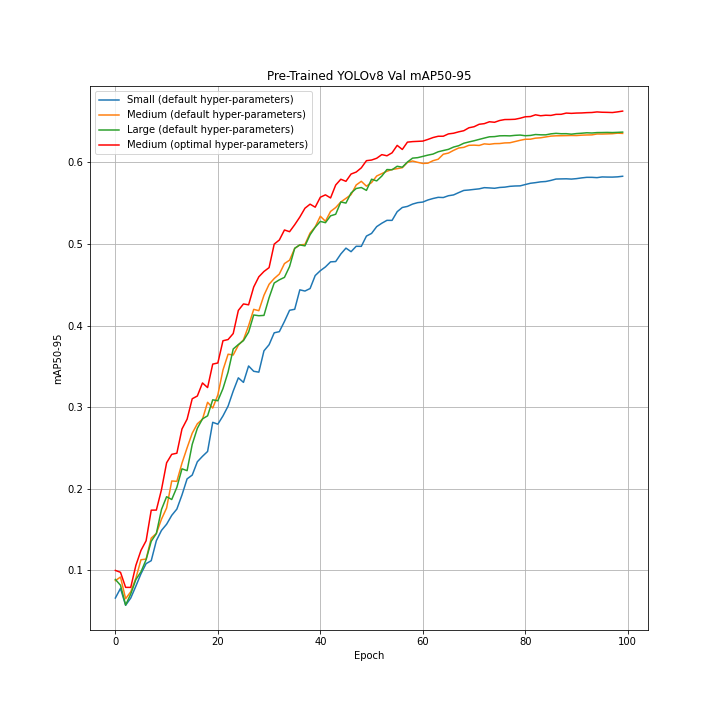
\includegraphics[width=0.4\textwidth]{figures/Pre-Trained YOLOv8 Val mAP50-95.png}
    \caption{Pre-Trained YOLOv8 Val mAP50-95}
    \label{fig:YOLOv8_mAP50-95_val}
\end{figure}
\begin{figure}
    \centering
    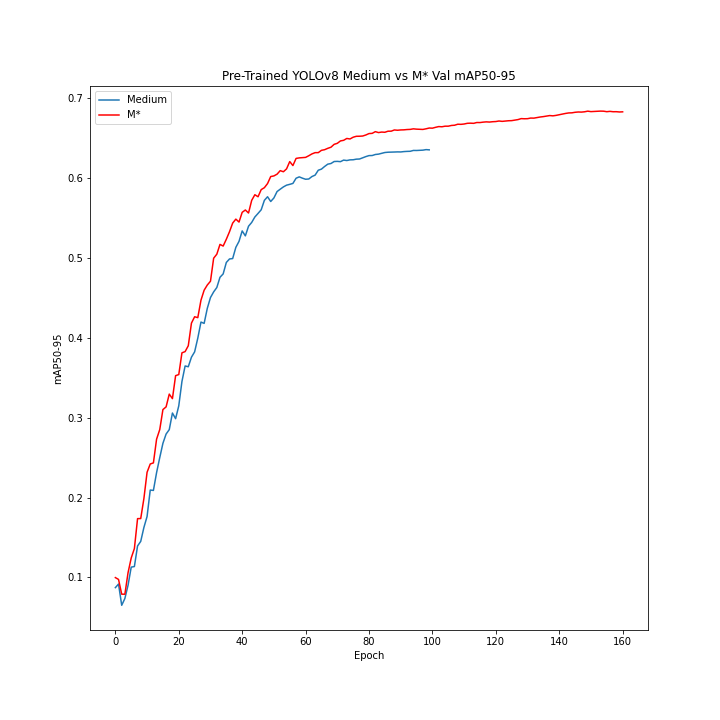
\includegraphics[width=0.4\textwidth]{figures/Pre-Trained YOLOv8 Medium vs Mstar Val mAP50-95.png}
    \caption{Pre-Trained YOLOv8 Medium vs Mstar Val mAP50-95}
    \label{fig:M_mAP50-95_val}
\end{figure}
\end{document}
